
\begin{document}
\pagenumbering{roman}
\title{COMS4040A \& COMS7045A Assignment 2 -- Report}
\author{Shameel Nkosi, 1814731, Coms Hons}
%\date{} 
\maketitle 
%\thispagestyle{empty}
\pagestyle{fancy}
\fancyhf{}
\fancyhead[R]{\thepage}
\fancyhead[L]{COMS4040A \& COMS7045A Assignment 2}
%\vskip 3mm 
%\pagenumbering{roman}
\newpage
\tableofcontents
\newpage
\begin{center}
	\textit{This page is intentionally left blank}
\end{center}
\newpage
\pagenumbering{arabic}
\section*{Introduction}
\addcontentsline{toc}{section}{Introduction}
\subsection*{Convolutions}
\addcontentsline{toc}{subsection}{Convolutions}
In this report I discuss convolutions an different implementations. Convolutions in the context of this report are nothing more than processing images digital. Convolutions can however, be applied to images, video or even audio. The goal to achieve the task of as quick as possible given that having a lot of computations can have notable performance issues.

The images we are reading in are gray-scale images. Each image being read has width and height. This means that there are pixels on the x-axis as well as the y-axis. Since the picture is gray-scale, each pixel has a single value instead of a \textit{rgb} vector of 3 values per pixel. This makes our job slightly easier. 

\subsection*{Design Style}
\addcontentsline{toc}{subsection}{Design Style}
\subsubsection*{Initial implementation}
 The images here are loaded as single array of values of size \textit{width} x \textit{height} instead of a 2 dimensional array of dimension \textit{(width,height)}. Initially, the design style I employed was one that worked on an \textit{n by m} matrix which worked pretty well and was easy to maintain and keep track of the indices. This however, required me to turn the loaded image into a two dimensional array and then back to a one dimensional upon being processed so that it can be written to a file. 
 
 \subsubsection*{Current implementation}
 In the implementation submitted, The code works on one dimensional arrays throughout. This makes reading and writing of images easy and it also enables one to avoid making mistakes of deforming the image. As required, there are 4 different implementations done here:
 \begin{itemize}
 	\item \textbf{Serial implementation:} In this implementation everything is done sequentially, one computation at a time by a single processor.
 	\item \textbf{Parallel with global and constant memory:} The parallel code is implemented using the CUDA programming interface. Here we have a number of threads working together to achieve a common goal, executing the same instruction on different parts of the memory. Memory here is on disk, therefore for every thread executing, the thread makes a request for an item in memory.
 	\item \textbf{Parallel with shared and constant memory:}  Similar to the point above with a small, here memory is shared and therefore cached. This means that if a block is shared, a request is made only once for a block of memory, threads sharing memory use the cached or fetched memory. This avoids the traffic to and from main memory. We therefore, expect this implementation to be better than the one above.
 	\item \textbf{Parallel with texture memory:} This is read only memory that aims to gives us better performance gains compared to any on the implementations mentioned above. Texture exploits the idea of spatial memory access, which states that if you access memory, you are likely to use the neighboring memory blocks, therefore when a request is made, neighboring memory comes with that requested memory address, which is what we need in the purposes of the our assignment.
 \end{itemize}

One will need to change the values in the code for different executions of the code. The code happens in two line. For default values, Change line 12 $maskChoice$ to: 
\begin{itemize}
	\item $1$ for average mask.
	\item $2$ for sharpening mask.
	\item $3$ for edge detection
	\item $4$ for average mask with kernel of size $5x5$
\end{itemize}

What else needs to change is the $imageFilename$ on line 26 and it can take the following values:
\begin{itemize}	
	\item For average mask
	\begin{itemize}
		\item "$image21/average/image21.pgm$"
		\item "$lena/average/lena_bw.pgm$"
		\item "$man/average/man.pgm$"
		\item "$mandrill/average/mandrill.pgm$"
	\end{itemize}	
	
	\item For sharpening mask
	\begin{itemize}
		\item "$image21/sharpening/image21.pgm$"
		\item "$lena/sharpening/lena_bw.pgm$"
		\item "$man/sharpening/man.pgm$"
		\item "$mandrill/sharpening/mandrill.pgm$"
	\end{itemize}	
	
	\item For edge detection mask
	\begin{itemize}
		\item "$image21/edge/image21.pgm$"
		\item "$lena/edge/lena_bw.pgm$"
		\item "$man/edge/man.pgm$"
		\item "$mandrill/edge/mandrill.pgm$"
	\end{itemize}

\end{itemize}

\section*{Performance}
\addcontentsline{toc}{section}{Performance}
\subsection*{Performance Comparisons Among All Approaches}
\addcontentsline{toc}{subsection}{Performance Comparisons Among All Approaches}
In this section we show the performance comparisons among all approaches but not for all pictures. The reason why I will not show for all pictures that were used in this assignment is because the all pictures were of the exact size and dimensions, and therefore the output for each we very similar. This will be proven by means of pictures or screenshots and then I will explain the results.

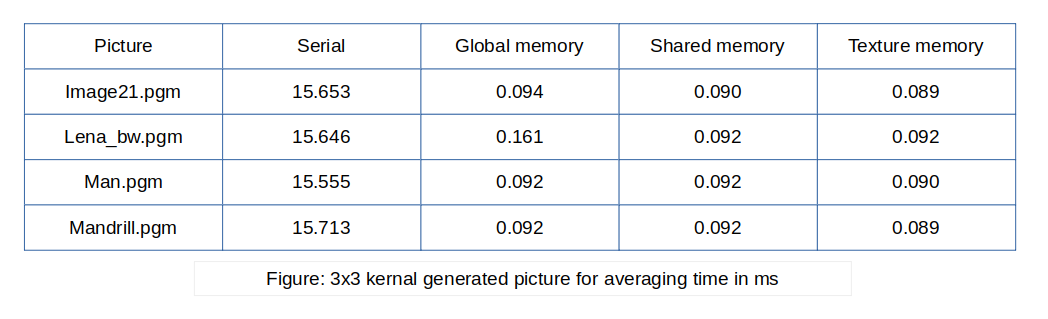
\includegraphics[scale=0.5]{Performance/averaging3.png}
\\
\textbf{Averaging: }Above are the times taken for each implementation per picture. With no doubt we can see that the Serial time is far far greater than any times tabulated. This is because every block or entry in memory for the output image is calculated one after the other.
We expect the texture memory results to be the best and with no doubt they are as expected and explained in the design styles section of this report. Though the differences aren't significantly different, shared memory outperforms global memory on average but not all time. Please note that the reasons mentioned here for performance will apply to the tables we are going to list below for other kernels.

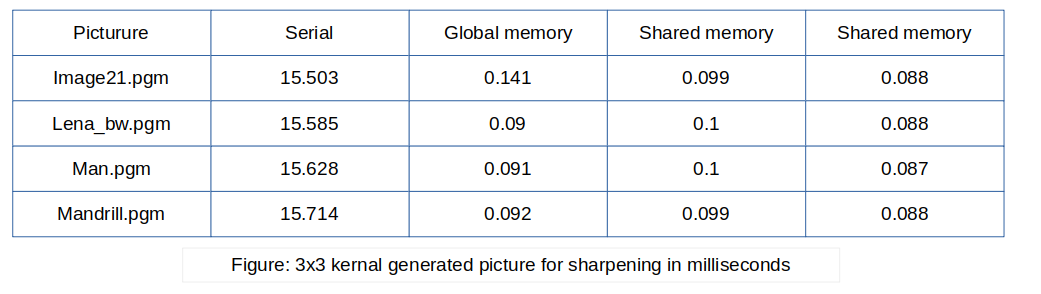
\includegraphics[scale=0.5]{Performance/sharpening.png}
\textbf{Sharpening: }Here we can conclude that serial time and texture time are living up to what we expect of them. Though shared memory is required to outperform global at all times, we fail to achieve that. The reason is due to the initialization of the tile size memory that has to be shared. This could however been optimized had I had more time to work on the code. 

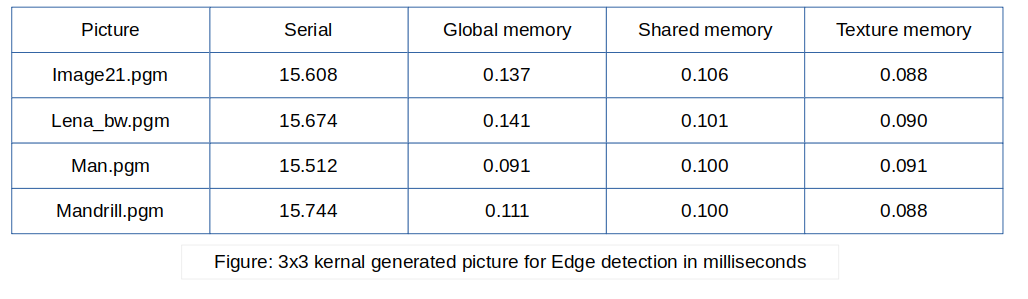
\includegraphics[scale=0.5]{Performance/edgeDetection.png}
\textbf{Edge Detection: }Again here we have results that we are expecting except for the man.pgm picture where the global memory out performs the Shared memory. This is fine however as we can agree that the shared memory is on average outperforming the global memory and the texture memory is outperforming any other implementation.
\\ \\ \\
\subsection*{Performance comparison of different size kernel}
\addcontentsline{toc}{subsection}{Performance comparison of different size kernel}
I will keep this section short. Below is the comparisons for kernels of dimension $(5 x 5)$, here the differences are significantly different and somewhat disappointing to and a certain degree. That is fine though because this is life and we don't always get what we want from it. With that said, hope life will favor me with good grades for this assignment :-).

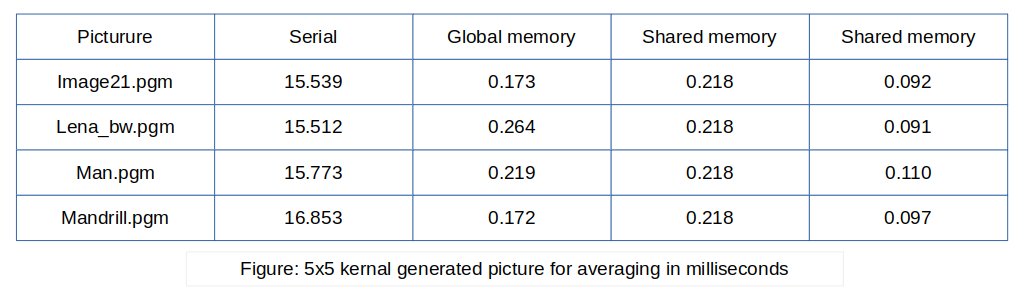
\includegraphics[scale=0.5]{Performance/averaging5.png}

\section*{Images}
\addcontentsline{toc}{section}{Images}
Below I show all the images that have been generated by the code. The format of these pictures will be as follows, each row will contain pictures generated in serial, global memory, shared memory and texture memory. Above each row will be the original picture for which it was Generated.

\subsection*{Averaging pictures}
I will however am going to show some pictures and not all due to me running out of time in compiling this report. To start of, below is the image of the papers.

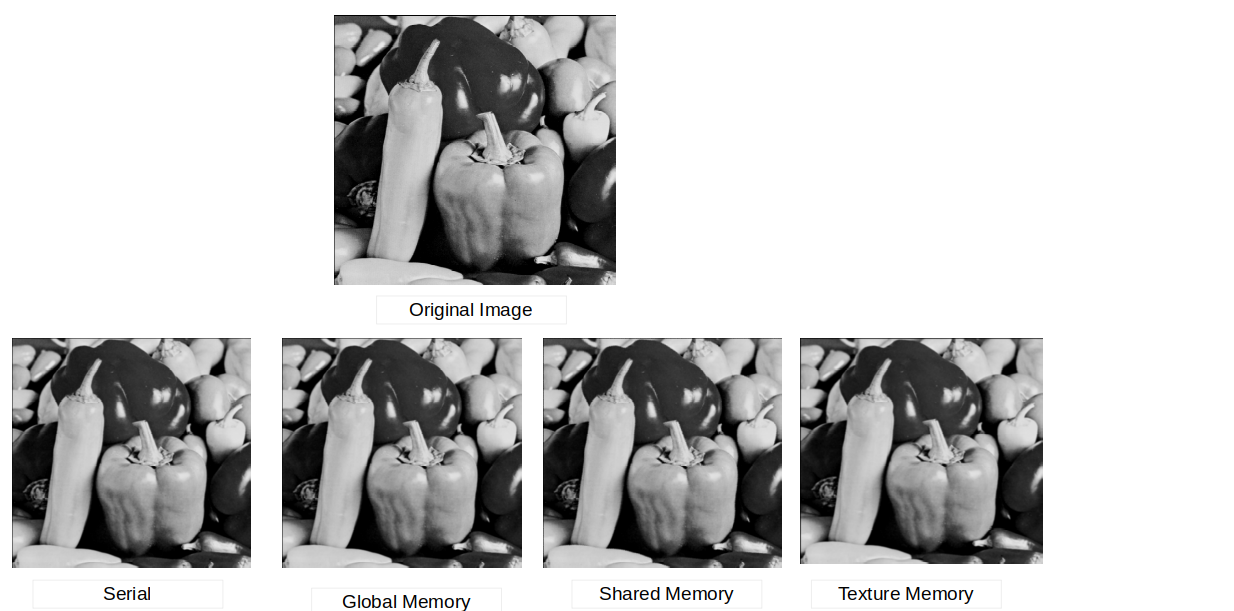
\includegraphics[scale=0.5]{images/image21Ave.png}
 
 \subsection*{Edge detection pictures}
 Here we show the results of edge detection using other pictures.
 
 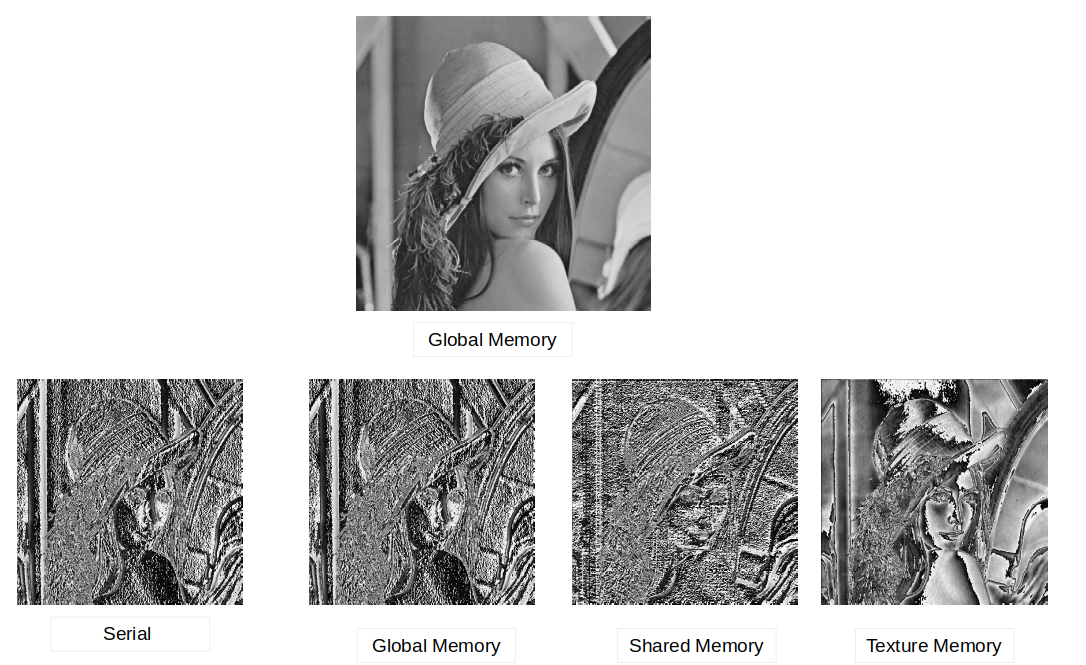
\includegraphics[scale=0.5]{images/lenaEdge.png}
 
  \subsection*{Sharpening pictures}
 Here we show the results of edge detection using other pictures.
 
  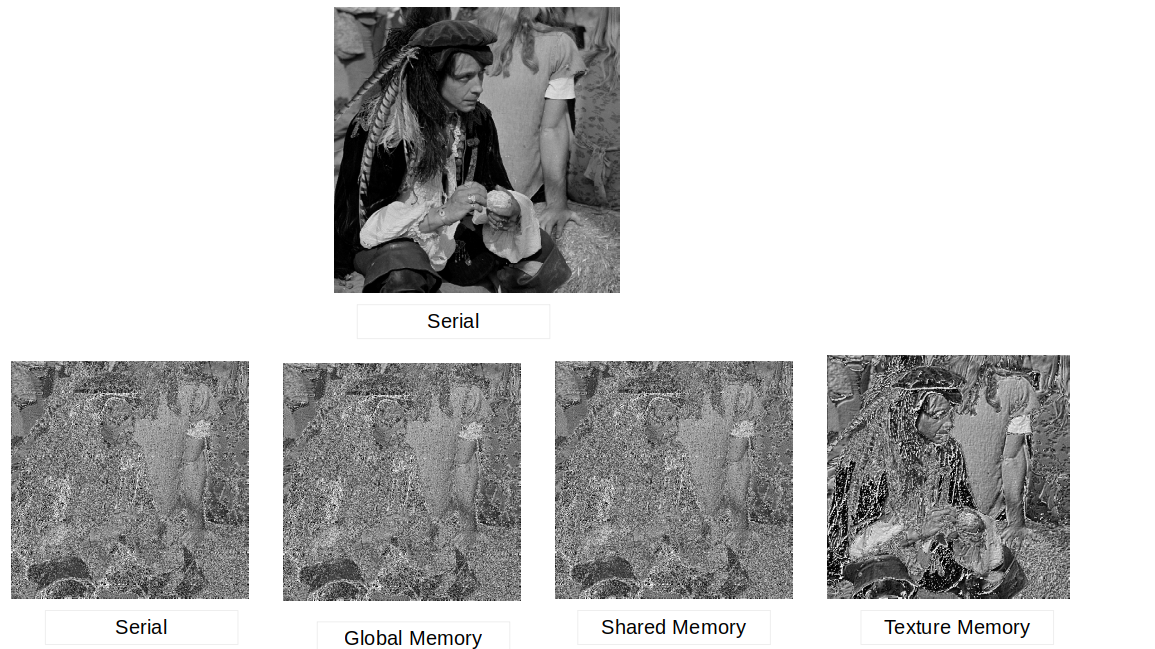
\includegraphics[scale=0.5]{images/manSharp.png}
  
 \section*{Conclusion}
 I believe the everything was as required and performance tables speak.

\end{document} 

